\documentclass[ektypwsh]{frontisthrio}
\usepackage[T1]{fontenc}
\usepackage[english,greek]{babel}
\usepackage{amsmath,rotate,tikz}
\usepackage{nimbusserif} % txfontsb,libertinus,libertine,kerkis,nimbusserif
\let\Bbbk\relax
\usepackage[amsbb,subscriptcorrection,zswash,mtpcal,mtphrb,mtpfrak]{mtpro2}
\newcommand{\kerkissans}[1]{{\fontfamily{maksf}\selectfont #1}}
\usetikzlibrary{decorations.pathreplacing,backgrounds}
\tkzSetUpPoint[size=2.8,fill=white]
%-----------------------
\usepackage[explicit]{titlesec}
\usepackage{sectsty}
\sectionfont{\centering}
\usepackage{graphicx,tabularx,fontawesome5,pgfplots,calc,tcolorbox,hhline,adjustbox,mathimatika,gensymb,eurosym,wrap-rl,systeme,regexpatch,mathtools,booktabs,calculator}
\let\vary\relax
\usepackage{exsheets,multicol}
%----------------------------
\tcbuselibrary{skins,theorems,breakable}
\tikzstyle{pl}=[line width=0.3mm]
\tikzstyle{plm}=[line width=0.4mm]
\usepackage{etoolbox}
\makeatletter
\renewrobustcmd{\anw@true}{\let\ifanw@\iffalse}
\renewrobustcmd{\anw@false}{\let\ifanw@\iffalse}\anw@false
\newrobustcmd{\noanw@true}{\let\ifnoanw@\iffalse}
\newrobustcmd{\noanw@false}{\let\ifnoanw@\iffalse}\noanw@false
\renewrobustcmd{\anw@print}{\ifanw@\ifnoanw@\else\numer@lsign\fi\fi}
\makeatother
\newcounter{method}[section]
\newcommand{\Method}[1]{\refstepcounter{method}{\bmath{{\Large \thesection}.\arabic{method} : #1}}}
\newlist{bhma}{enumerate}{3}
\setlist[bhma]{label=\bf\textit{\arabic*\textsuperscript{o}\;Βήμα :},leftmargin=1cm,itemindent=1cm,ref=\bf{\arabic*\textsuperscript{o}\;Βήμα}}
\newlist{tropos}{enumerate}{3}
\setlist[tropos]{label=\bf\textit{\arabic*\textsuperscript{oς}\;Τρόπος :},leftmargin=0cm,itemsep=0mm,itemindent=2cm,ref=\bf{\arabic*\textsuperscript{oς}\;Τρόπος}}
\newcommand{\en}[1]{{\selectlanguage{english}#1\selectlanguage{greek}}}
\newlist{periptwsh}{enumerate}{3}
\setlist[periptwsh]{label=\bf\textit{\arabic*\textsuperscript{oς}\;Περίπτωση :},leftmargin=0cm,itemsep=0mm,itemindent=2.8cm,ref=\bf{\arabic*\textsuperscript{oς}\;Περίπτωση}}

\begin{document}
\section{Σύνθεση συναρτήσεων}
\Method{Εύρεση σύνθεσης}\\
Για να οριστεί η συνάρτηση $ f\circ g $ πρέπει να βρούμε το πεδίο ορισμού της και τον τύπο της για κάθε $ x\in D_{f\circ g} $
\begin{bhma}
\item Για το πεδίο ορισμού ισχύουν οι σχέσεις
\[ x\in D_g\ \ \textrm{ και }\ \ g(x)\in D_f \]
Οι περιορισμοί αυτοί μα οδηγούν σε εξισώσει και ανισώσεις των οποίων οι κοινές λύσεις σχηματίζουν το πεδίο ορισμού.
\item Ο τύπος της $ f\circ g $ θα ισούται με
\[ (f\circ g)(x)=f(g(x)) \]
που σημαίνει ότι στον τύπο της $ f $ αντικαθιστούμε το $ x $ με $ g(x) $.
\end{bhma}
Εντελώς ανάλογα εργαζόμαστε για τις συναρτήσεις $ g\circ f, f\circ f\ldots $
\newpage\section{Συνάρτηση $ 1-1 $ - Αντίστροφη}
\Method{Συνάρτηση $ 1-1 $}\\
Υπάρχουν οι εξής τρόποι για να αποδείξουμε ότι μια συνάρτηση $ f:D_f\to\mathbb{R} $ είναι $ 1-1 $.
\begin{tropos}
\item Αποδεικνύοντας ότι η $ f $ είναι γνησίως μονότονη στο $ D_f $. (Ο τρόπος αυτός ενδείκνυται όταν το πεδίο ορισμού της $ f $ είναι ένα διάστημα.)
\item Με τη βοήθεια του ορισμού της $ 1-1 $ συνάρτησης
\[ \textrm{Για κάθε }x_1,x_2\in D_f \ \ : \ \  f(x_1)=f(x_2)\Rightarrow x_1=x_2 \]
(Ο τρόπος αυτός ενδείκνυται για συναρτήσεις με πεδίο ορισμού ένωση διαστημάτων, αρκεί ο τύπος να επιτρέπει την επίλυση της εξίσωσης.)
\item Με τη βοήθεια της γραφικής παράστασης της $ f $. Κάθε οριζόντια ευθεία πρέπει να τέμνει τη $ C_f $ σε ένα το πολύ σημείο.
\item Αν η εξίσωση $ y=f(x) $ έχει μοναδική λύση ως προς $ x $ για κάθε $ y\in f(D_f) $ και η λύση ανήκει στο $ D_f $ τότε η $ f $ είναι $ 1-1 $.
\item Με απαγωγή σε άτοπο. Υποθέτουμε δηλαδή ότι η $ f $ δεν είναι $ 1-1 $.
\end{tropos}
\begin{flushright}
\begin{minipage}{7cm}
\textit{Πηγή: Μαθηματικά Γ΄ Λυκείου, Η επανάληψη. Ανδρέας Πάτσης - Παύλος Τρύφων, Εκδόσεις Ελληνοεκδοτική}
\end{minipage}
\end{flushright}
\Method{Εύρεση αντίστροφης συνάρτησης}
\begin{multicols}{2}
\begin{tropos}
\item\mbox{}\\\vspace{-7mm}
\begin{bhma}
\item Εύρεση συνόλου τιμών της $ f $ με τη βοήθεια μονοτονίας.
\item Επίλυση της εξίσωσης $ y=f(x) $ ως προς $ x $ με $ x\in D_f $.
\end{bhma}
\vspace{4mm}
\item\mbox{}\\\vspace{-7mm}
\begin{bhma}
\item Επίλυση της εξίσωσης $ y=f(x) $ ως προς $ x $ με $ x\in D_f $.
\item Κατά τη διάρκεια επίλυσης της παραπάνω εξίσωσης, παίρνουμε περιορισμούς που αφορούν τη μεταβλητή $ y $. Όταν λυθεί ως προς $ x $ επιπλέον περιορισμός είναι $ x\in D_f $.
\end{bhma}
\end{tropos}
\end{multicols}
\newpage\section{Όρια}
Οι απροσδιόριστες μορφές που μπορεί να έχει ένα όριο είναι οι ακόλουθες :
\begin{alist}
\item Μορφή κλάσματος : $ \dfrac{0}{0} $ και $ \dfrac{\pm\infty}{\pm\infty} $
\item Μορφή γινομένου : $ 0\cdot(\pm\infty) $
\item Μορφή δύναμης : $ 0^0,1^{\pm\infty},(\pm\infty)^0 $
\item Μορφή αθροίσματος : $ \infty-\infty $
\end{alist}
Θα μελετήσουμε επίσης τη μορφή $ \frac{a}{0} $.\\\\
\Method{Όρια με απροσδιοριστία $ \frac{0}{0} $}
\begin{Alist}
\begin{multicols}{2}
\item Με ρητή συνάρτηση
\begin{tropos}
\item Παραγοντοποίηση
\item Κανόνας \en{De L'Hospital}
\end{tropos}
\item Με ρίζες :\\Πολλαπλασιασμός με συζυγείς παραστάσεις.
\end{multicols}
\item Με απόλυτες τιμές
\begin{bhma}
\item Υπολογίζω τα όρια των παραστάσεων μέσα στις απόλυτες τιμές.
\item Διώχνω τις απόλυτες τιμές με τον παρακάτω κανόνα
\begin{gather*}
\lim_{x\to x_0}{f(x)}>0\Rightarrow f(x)>0\ \textrm{κοντά στο }x_0\\
\lim\limits_{x\to x_0}{f(x)}<0\Rightarrow f(x)<0\  \textrm{κοντά στο }x_0
\end{gather*}
Αν κάποια απόλυτη τιμή μηδενίζεται στο $ x_0 $ τότε υπολογίζω πλευρικά όρια.
\item Υπολογίζω όριο ρητής $ \frac{0}{0} $
\end{bhma}
\item Με τριγωνομετρικές παραστάσεις
\begin{tropos}
\item Κατασκευάζω και χρησιμοποιώ τριγωνομετρικές ταυτότητες.
\item Κατασκευάζω με πράξεις κάποιο βασικό τριγωνομετρικό όριο, αρκεί όταν $ x\to x_0 $ να μηδενίζεται η γωνία του τριγωνομετρικού αριθμού.
\item Κανόνας \en{De L' Hospital}. (Χρειάζεται προσοχή εδώ γιατί μπορεί η εφαρμογή του κανόνα να με οδηγήσει σε δυσκολότερο όριο.)
\end{tropos}
\item Με εκθετικές, λογαριθμικές και συνδυασμό αυτών : Κανόνας \en{De L' Hospital}
\end{Alist}
\Method{Όρια με απροσδιοριστία $ \frac{\infty}{\infty} $}
\begin{Alist}
\item Με ρητή συνάρτηση όταν $ x\to\infty $ υπολογίζουμε το όριο του κλάσματος μόνο με τους μεγιστοβάθμιους όρους.
\item Με ρίζες : Μέθοδος κοινού παράγοντα.
\item Διάφορες συναρτήσεις : Κανόνας \en{De L' Hospital}
\end{Alist}
\Method{Όρια με απροσδιοριστία $ 0\cdot(\pm\infty) $}
\begin{bhma}
\item Γράφουμε το γινόμενο με μορφή σύνθετου κλάσματος ως εξής
\[ \lim_{x\to x_0}{\left(f(x)\cdot g(x)\right)}=\lim_{x\to x_0}{\dfrac{f(x)}{\frac{1}{g(x)}}}\ \ \textrm{ή}\ \ \lim_{x\to x_0}{\dfrac{g(x)}{\frac{1}{f(x)}}} \]
\item Το όριο παίρνει τη μορφή $ \dfrac{0}{0} $ ή $ \dfrac{\infty}{\infty} $ οπότε εφαρμόζουμε κανόνα \en{De L' Hospital}
\end{bhma}
\Method{Όρια με απροσδιοριστία $ 0^0,1^{\pm\infty},(\pm\infty)^0 $}
\begin{bhma}
\item Χρησιμοποιούμε τον παρακάτω κανόνα
\[ \lim_{x\to x_0}{f(x)^{g(x)}}=\lim_{x\to x_0}{e^{\ln{f(x)^{g(x)}}}}=\lim_{x\to x_0}{e^{g(x)\cdot\ln{f(x)}}} \]
\item Υπολογίζουμε το όριο του εκθέτη το οποίο έχει απροσδιοριστία $ 0\cdot(\pm\infty) $. Στη συνέχεια με αντικατάσταση υπολογίζουμε το αρχικό όριο.
\end{bhma}
\Method{Όρια με απροσδιοριστία $ \infty-\infty $}\\
Για τον υπολογισμό ορίου $ \lim\limits_{x\to x_0}{(f(x)-g(x))} $ με απροσδιοριστία $ \infty-\infty $ ακολουθούμε έναν από τους παρακάτω τρόπους:
\begin{tropos}
\item Βγάζουμε κοινό παράγοντα μια από τις δύο συναρτήσεις.
\[ \lim_{x\to x_0}{(f(x)-g(x))}=\lim_{x\to x_0}{f(x)\left[1-\frac{g(x)}{f(x)}\right]} \]
Στη συνέχεια υπολογίζουμε το όριο του κλάσματος $ \frac{g(x)}{f(x)} $ με μορφή $ \infty-\infty $.
\item Αν οι $ f(x),g(x) $ είναι κλάσματα, τα κάνουμε ομώνυμα.
\item Σχηματίζουμε διαφορά λογαρίθμων και χρησιμοποιούμε την ιδιότητα
\[ \ln{a}-\ln{\beta}=\ln{\frac{a}{\beta}} \]
Στη συνέχεια υπολογίζουμε το όριο του κλάσματος.
\end{tropos}
\Method{Όρια της μορφής $ \frac{a}{0} $}
\begin{bhma}
\item Παραγοντοποιούμε τον παρονομαστή.
\item Γράφουμε σε ξεχωριστό κλάσμα τον παράγοντα που μηδενίζεται.
\item Αν αυτός ο παράγοντας έχει σταθερό πρόσημο τότε προχωράμε στον υπολογισμό. Αν όχι υπολογίζουμε πλευρικά όρια.
\end{bhma}
\Method{Όρια με τριγωνομετρικές συναρτήσεις $ \hm{f(x)},\syn{f(x)} $ - Μηδενική επί φραγμένη}\\
Αν το όριο περιέχει σύνθετες τριγωνομετρικές συναρτήσεις με γωνία $ f(x) $ και $ \lim\limits_{x\to x_0}{f(x)}=\pm\infty $ τότε
\begin{bhma}
\item Γράφουμε τη συνάρτηση μέσα στο όριο ως γινόμενο συναρτήσεων. 
\item Κλείνουμε τη συνάρτηση του ορίου σε απόλυτη τιμή και σχηματίζουμε διπλή ανισότητα ώστε να εφαρμοστεί κριτήριο παρεμβολής.
\end{bhma}
\Method{Γνωστό όριο που περιέχει την $ f(x) $ - Βοηθητική συνάρτηση}
\begin{bhma}
\item Θέτουμε $ g(x) $ τη συνάρτηση του ορίου και λύνουμε ως προς $ f(x) $.
\item Υπολογίζουμε το όριο της $ f $ στο $ x_0 $.
\end{bhma}
\Method{Κριτήριο παρεμβολής}\\
Το κριτήριο παρεμβολής για τον υπολογισμό ορίων εφαρμόζεται σε ανισότητες της μορφής
\[ g(x)\leq f(x)\leq h(x)\ \ \textrm{ή}\ \ |f(x)|\leq g(x)\Rightarrow -g(x)\leq f(x)\leq g(x) \]
\newpage\section{Εφαπτομένη}
\Method{Εύρεση εφαπτομένης με γνωστό σημείο επαφής}
\begin{bhma}
\item Πεδίο ορισμού, παράγωγος $ f' $ και θέτουμε όπου $ x=x_0 $ ώστε να βρεθούν οι αριθμοί $ x_0,f(x_0) $ και $ f'(x_0) $.
\item Γράφουμε την εξίσωση της ευθείας
\[ y-f(x_0)=f'(x_0)(x-x_0) \]
και αντικαθιστώντας λύνουμε ως προς $ y $.
\end{bhma}
\Method{Εύρεση εφαπτομένης με γνωστή κλίση λ}
\begin{bhma}
\item Πεδίο ορισμού και $ f' $.
\item Θεωρούμε σημείο επαφής $ M(x_0,f(x_0)) $ και θέτουμε το σ.δ. της εφαπτομένης να ισούται με τη δοσμένη κλίση $ \lambda $.
\[ f(x_0)=\lambda \]
Αν δεν μας δίνεται ο συντελεστής $ \lambda $ της εφαπτομένης $ \varepsilon $ τότε τον βρίσκουμε έχοντας τις εξής περιπτώσεις.
\begin{center}
\begin{tabular}{c|c}
\hline
\rule[-2ex]{0pt}{5.5ex} \textbf{Συνθήκη} & \textbf{Εξίσωση} \\
\hhline{==}
\rule[-2ex]{0pt}{5.5ex} Ευθείες παράλληλες $ \varepsilon\parallel \zeta $ &$ \lambda_{\varepsilon}=\lambda_{\zeta}\Rightarrow f'(x_0)=\lambda $  \\
\hline
\rule[-2ex]{0pt}{5.5ex} Ευθείες κάθετες $ \varepsilon\perp\zeta $ & $ \lambda_{\varepsilon}\cdot\lambda_{\zeta}=-1\Rightarrow \ldots\Rightarrow f'(x_0)=\lambda $ \\
\hline
\rule[-2ex]{0pt}{5.5ex} Οριζόντια ευθεία $ \varepsilon\parallel x'x $  & $ \lambda_{\varepsilon}=0\Rightarrow f'(x_0)=0 $ \\
\hline
\rule[-2ex]{0pt}{5.5ex} Η $ \varepsilon $ σχηματίζει γωνία $ \omega $ & $ \lambda_{\varepsilon}=\ef{\omega}\Rightarrow f'(x_0)=\ef{\omega} $. \\
\hline
\end{tabular}
\end{center}
\item Λύνουμε την εξίσωση, βρίσκουμε το $ x_0 $ και στη συνέχεια το $ f(x_0) $.
\item Εξίσωση ευθείας $ y-f(x_0)=f'(x_0)(x-x_0) $.
\end{bhma}
\Method{Εφαπτομένη που διέρχεται από εξωτερικό σημείο $ P(a,\beta) $}
\begin{bhma}
\item Πεδίο ορισμού και $ f' $.
\item Θεωρούμε σημείο επαφής $ M(x_0,f(x_0)) $ και γράφουμε τον τύπο της ευθείας.
\item Αντικαθιστούμε $ f(x_0) $ και $ f'(x_0) $ στην εξίσωση.
\item Αφού $ P\in\varepsilon $ τότε θέτουμε $ x=a $ και $ y=\beta $ και λύνουμε την εξίσωση ως προς $ x_0 $.
\item Για κάθε $ x_0 $ υπολογίζουμε $ f(x_0) $ και $ f'(x_0) $ και βρίσκουμε την ευθεία.
\end{bhma}
\Method{Ευθεία εφάπτεται στη $ C_f $ στο $ M(x_0f(x_0)) $}
\[ \textrm{Η ευθεία }y=ax+\beta\textrm{ εφάπτεται στη }C_f\Leftrightarrow \ccases{f(x_0)=ax_0+\beta\\f'(x_0)=a} \]
\Method{Κοινή εφαπτομένη $ C_f,C_g $ σε κοινό σημείο $ M(x_0,f(x_0)) $}
\[ \textrm{Οι }C_f\textrm{ και }C_g\textrm{ έχουν κοινή εφαπτομένη στο }Μ\Leftrightarrow \ccases{f(x_0)=g(x_0)\\f'(x_0)=g'(x_0)} \]
\newpage\section{Ρυθμός μεταβολής}
\Method{Εύρεση ρυθμού μεταβολής συνάρτησης}
\begin{bhma}
\item Δίνουμε ονόματα στις συναρτήσεις του προβλήματος, προσέχοντας ποια είναι η ανεξάρτητη μεταβλητή.
\item Γράφουμε τα στοιχεία του προβλήματος με σύμβολα. Προσέχουμε στους ρυθμούς μεταβολής να βάλουμε το σωστό πρόσημο.
\item Γράφουμε τον κατάλληλο τύπο που περιέχει τη ζητούμενη συνάρτηση, ώστε παραγωγίζοντας να εμφανιστεί ο ρυθμός μεταβολής της.
\item Αν το πρόβλημα ζητάει παράγωγο σε σημείο (π.χ. σε κάποια χρονική στιγμή)  συμβολίσουμε με $ x_0,t_0\ldots $ το σημείο αυτό και θέτουμε $ x=x_0, t=t_0\ldots $ στον τύπο της παραγώγου.*
\end{bhma}
*Αν η ζητούμενη παράγωγος δεν είναι ο μοναδικός άγνωστος, πρέπει να γράψουμε κι άλλον τύπο ώστε να υπολογίσουμε τους άγνωστους που μας εμποδίζουν.\\\\
Στον παρακάτω πίνακα βλέπουμε τύπος για την περίμετρο και το εμβαδόν επίπεδων σχημάτων καθώς και τύπους για εμβαδόν και όγκο τρισδιάστατων στερεών.
\begin{center}
\begin{tabular}{c|c|c||c|c|c}
\hline
\rule[-2ex]{0pt}{5.5ex}  & \textbf{Περίμετρος} & \textbf{Εμβαδόν} & & \textbf{Εμβαδόν} & \textbf{Όγκος} \\
\hhline{======}
\rule[-2ex]{0pt}{5.5ex} Τετράγωνο &$ \Pi=4a $  & $ E=a^2 $ &Κύβος & $ E=6a^2 $ & $ V=a^3 $ \\
\hline
\rule[-2ex]{0pt}{5.5ex} Ορθογώνιο & $ \Pi=2(\mu+\pi) $ & $ E=\mu\pi$ & Παραλλ/δο & $ E=2(a\beta+\beta\gamma+a\gamma) $ &$ V=a\beta\gamma $  \\
\hline
\rule[-2ex]{0pt}{5.5ex} Παραλλ/μο & $ \Pi=2(a+\beta) $ & $ E=\beta\upsilon $ &Κύλινδρος & $ E=2\pi\rho h+2\pi\rho^2 $ & $ V=\pi\rho^2h $ \\
\hline
\rule[-2ex]{0pt}{5.5ex} Τρίγωνο & $ \Pi=a+\beta+\gamma $ & $ E=\frac{\beta\upsilon}{2} $ &Κώνος &$ E=\pi\rho\lambda+\pi\rho^2 $  & $ V=\frac{1}{3}\pi\rho^2h $ \\
\hline
\rule[-2ex]{0pt}{5.5ex} Τραπέζιο & $ \Pi=a+\beta+\gamma+\delta $ & $ E=\frac{(B+\beta)\upsilon}{2} $ &Σφαίρα & $ E=4\pi\rho^2 $ & $ V=\frac{4}{3}\pi\rho^3 $ \\
\hline
\rule[-2ex]{0pt}{5.5ex} Κύκλος & $ \Pi=2\pi\rho $ &$ E=\pi\rho^2 $ &Πυραμίδα &$ E=\ldots E_{\beta} $ & \\
\hline
\end{tabular}
\end{center}
\newpage\section{Μονοτονία - Ακρότατα}
\Method{Εύρεση μονοτονίας - ακρότατων - συνόλου τιμών - πλήθος ριζών συνάρτησης}
\begin{bhma}
\item Πεδίο ορισμού της $ f $ και έλεγχος συνέχειας
\item Παράγωγος $ f' $.
\item Υπολογίζουμε τις ρίζες και τα πρόσημα της $ f' $ με έναν από τους παρακάτω τρόπους :
\begin{itemize}
\item Λύνοντας την εξίσωση $ f(x)=0 $  και τις ανισώσεις $ f(x)>0 $ και $ f(x)<0 $.
\item Με επιλογή τιμής σε κάθε διάστημα που χωρίζουν οι ρίζες το πεδίο ορισμού. Οι ρίζες βρίσκονται και εδώ λύνοντας την εξίσωση $ f(x)=0 $.
\item Παραγωγίζοντας δεύτερη ή ακόμα και τρίτη φορά. Με τη μονοτονία κάθε παραγώγου βρίσκουμε τα πρόσημά της ώσπου να φτάσουμε στη μονοτονία της $ f $. Οι ρίζες βρίσκονται με δοκιμές.
\end{itemize}
\item Σχεδιάζουμε πίνακα με τα πρόσημα της παραγώγου και τη μονοτονία της $ f $. (Συμπληρώνουμε αν χρειαστεί και επιπλέον γραμμές για τις ανώτερης τάξης παραγώγους που βρήκαμε.)
\item\mbox{}\\\vspace{-7mm}
\begin{center}
\begin{tabular}{|p{5cm}|p{5cm}|p{5cm}|}
\hline
\rule[-2ex]{0pt}{5.5ex} \textbf{Για εύρεση μονοτονίας} & \textbf{Για εύρεση ακροτάτων} & \textbf{Για εύρεση συνόλου τιμών} \\
\hline
\rule[-2ex]{0pt}{5.5ex} Αναφέρουμε το είδος της μονοτονίας σε κάθε διάστημα ξεχωριστά. & Ελέγχουμε για ακρότατα στα κρίσιμα σημεία και στα κλειστά άκρα του πεδίου ορισμού & Βρίσκουμε τις εικόνες των διαστημάτων μονοτονίας και τις ενώνουμε \\
\hline
\end{tabular}
\end{center}
\item Για την εύρεση του πλήθους ριζών της συνάρτησης, ελέγχουμε αν το $ 0 $ ανήκει στην εικόνα κάθε διαστήματος. Αναλυτικά
\[ 0\in f(\Delta_1)\Rightarrow \textrm{Υπάρχει }x_0 : f(x_0)=0 \]
Η ρίζα αυτή είναι μοναδική μέσα στο κάθε διάστημα γιατί η $ f $ είναι γνησίως μονότονη.
\end{bhma}
\newpage\section{Κυρτότητα - Σημεία καμπής}
\Method{Εύρεση κυρτότητας - σημείων καμπής}
\begin{bhma}
\item Πεδίο ορισμού και έλεγχος συνέχειας.
\item Υπολογίζουμε την δεύτερη παράγωγο $ f'' $.
\item Βρίσκουμε ρίζες και πρόσημα της $ f'' $ με τους τρόπους που περιγράψαμε στη μονοτονία.
\item Σχηματίζουμε πίνακα με τα πρόσημα της $ f'' $ και την κυρτότητα της $ f $.
\item \mbox{}\\\vspace{-7mm}
\begin{center}
\begin{tabular}{|p{7cm}|p{7cm}|}
\hline
\rule[-2ex]{0pt}{5.5ex} \textbf{Για εύρεση κυρτότητας} & \textbf{Για εύρεση σημείων καμπής} \\
\hline
\rule[-2ex]{0pt}{5.5ex} Αναφέρουμε το είδος της κυρτότητας σε κάθε διάστημα ξεχωριστά. & Ελέγχουμε για σημεία καμπής στα σημεία που αλλάζει η κυρτότητα αρκεί η $ f $ να είναι μια φορά παραγωγίσιμη στα σημεία αυτά. \\
\hline
\end{tabular}
\end{center}
\end{bhma}
\Method{Κυρτότητα και εφαπτομένες - Απόδειξη ανισότητας}
\begin{bhma}
\item Μελετάμε τη συνάρτηση ως προς την κυρτότητα.
\item Βρίσκουμε την εξίσωση της εφαπτομένης στο σημείο που ζητάει ή σε κάποιο σημαντικό σημείο. Αυτή θα έχει τη μορφή $ y=ax+\beta $
\item Χρησιμοποιούμε μια από τις παρακάτω σχέσεις
\[ f\rotatebox[origin=c]{180}{$ \curvearrowleft $}\Delta\Rightarrow f(x)\geq ax+\beta\ \ ,\ \ f\curvearrowright\Delta\Rightarrow f(x)\leq ax+\beta \]
και με πράξεις φέρνουμε την ανισότητα στη μορφή που τη ζητάει η άσκηση.
\end{bhma}
\newpage\section{Ασύμπτωτες}
\Method{Κατακόρυφες ασύμπτωτες}
\begin{bhma}
\item Πεδίο ορισμού της $ f $.
\item Υπολογισμός κάποιου πλευρικού ορίου στα σημεία $ x_0 $ που είναι ανοικτά άκρα του πεδίου ορισμού της $ f $ ή στα σημεία που δεν είναι συνεχής η συνάρτηση.
\item Αν κάποιο πλευρικό όριο ισούται με $ \pm\infty $ τότε η ευθεία $ x=x_0 $ είναι κατακόρυφη ασύμπτωτη της $ C_f $.
\end{bhma}
\Method{Οριζόντια ασύμπτωτη}
\begin{bhma}
\item Όριο της $ f $ στο $ +\infty $ ή $ -\infty $ εφόσον ορίζεται η $ f $ σε διάστημα που περιέχει $ \pm\infty $.
\item Αν $ \lim\limits_{x\to \pm\infty}{f(x)}=l $ τότε η ευθεία $ y=l $ είναι οριζόντια ασύμπτωτη της $ C_f $ στο $ \pm\infty $.
\end{bhma}
\Method{Πλάγια ασύμπτωτη}
\begin{bhma}
\item Εφόσον ορίζεται η $ f $ σε διάστημα που περιέχει $ \pm\infty $ υπολογίζουμε τα παρακάτω όρια.
\[ \lim_{x\to +\infty}{\frac{f(x)}{x}}=\lambda\ \ ,\ \ \lim_{x\to +\infty}{(f(x)-\lambda x)}=\beta \]
και αντίστοιχα στο $ -\infty $.
\item Αν $ \lambda\in\mathbb{R} $ και $ \beta\in\mathbb{R} $ τότε η ευθεία $ y=\lambda x+\beta $ είναι πλάγια ασύμπτωτη της $ C_f $ στο $ \pm\infty $.
\end{bhma}
\Method{Ασύμπτωτες γενικά}
\begin{bhma}
\item Αναζητούμε για κατακόρυφες ασύμπτωτες στα σημεία που αναφέραμε.
\item Ανάμεσα σε πλάγιες και οριζόντιες ασύμπτωτες, ξεκινάμε με τις πλάγιες και από το συντελεστή διεύθυνσης $ \lambda $ θα εξαρτηθεί αν η ευθεία είναι πλάγια ή οριζόντια. Ακολουθούμε το παρακάτω διάγραμμα:
\end{bhma}
\begin{center}
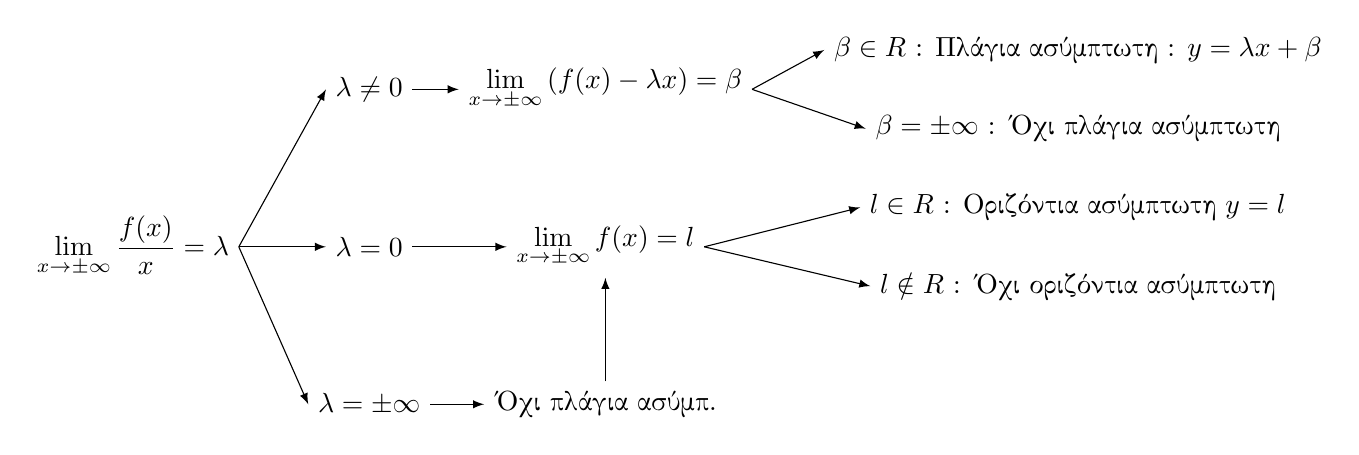
\begin{tikzpicture}
\node(a) at(-2,0){$ \lim\limits_{x\to\pm\infty}{\dfrac{f(x)}{x}}=\lambda $};
\node(b) at(1,2){$ \lambda\neq0 $};
\node(c) at(1,0){$ \lambda=0 $};
\node(d) at(1,-2){$ \lambda=\pm\infty $};
\node(e) at(4,2){$ \lim\limits_{x\to\pm\infty}{(f(x)-\lambda x)}=\beta $};
\node(f) at(10,2.5){$ \beta\in\mathbb{R} $ : Πλάγια ασύμπτωτη : $ y=\lambda x+\beta $};
\node(g) at(10,1.5){$ \beta=\pm\infty $ : Όχι πλάγια ασύμπτωτη};
\node(j) at(4,0){$ \lim\limits_{x\to \pm\infty}{f(x)}=l $};
\node(k) at(10,.5){$ l\in\mathbb{R} $ : Οριζόντια ασύμπτωτη $ y=l $};
\node(l) at(10,-.5){$ l\notin\mathbb{R} $ : Όχι οριζόντια ασύμπτωτη};
\node(m) at(4,-2){Όχι πλάγια ασύμπ.};
\draw[-latex] (a.0)--(b.180);
\draw[-latex] (a.0)--(c.180);
\draw[-latex] (a.0)--(d.180);
\draw[-latex] (b.0)--(e.180);
\draw[-latex] (e.0)--(f.180);
\draw[-latex] (e.0)--(g.180);
\draw[-latex] (j.0)--(k.180);
\draw[-latex] (j.0)--(l.180);
\draw[-latex] (d.0)--(m.180);
\draw[-latex] (c.0)--(j.180);
\draw[-latex] (m.90)--(j.270);
\end{tikzpicture}
\end{center}
\newpage
\section{Εύρεση παραμέτρων}
Η γενική μέθοδος για την εύρεση μιας παραμέτρου είναι να κατασκευάσουμε μια εξίσωση ή ανίσωση που να την περιέχει, ώστε λύνοντάς την να την προσδιορίσουμε. Κάποια συνθήκη της υπόθεσης είναι αυτή που θα μας οδηγήσει σ' αυτή την εξίσωση-ανίσωση. 
\begin{center}
\begin{tabular}{p{7.5cm}|p{7.5cm}}
\hline
\rule[-2ex]{0pt}{5.5ex} \textbf{Συνθήκη} & \textbf{Εξίσωση - Ανίσωση} \\
\hhline{==}
\rule[-2ex]{0pt}{5.5ex} Το σημείο $ A(a,\beta) $  ανήκει στη $ C_f $ & $ f(a)=\beta $ \\
\hline
\rule[-2ex]{0pt}{5.5ex} Γνωστό όριο που περιέχει παραμέτρους $ a,\beta\ldots $ & Βοηθητική συνάρτηση \\
\hline
\rule[-2ex]{0pt}{5.5ex} Η $ f $ είναι συνεχής σε σημείο $ x_0\in D_f $ & $ \lim\limits_{x\to x_0}f(x)=f(x_0) $ \\
\hline
\rule[-1ex]{0pt}{5.5ex} Η $ f $ είναι παραγωγίσιμη σε σημείο $ x_0\in D_f $ & $ \lim\limits_{x\to x_0^-}{\dfrac{f(x)-f(x_0)}{x-x_0}}=\lim\limits_{x\to x_0^+}{\dfrac{f(x)-f(x_0)}{x-x_0}} $ \\
\hline
\rule[0ex]{0pt}{5ex} Η ευθεία $ y=ax+\beta $ εφάπτεται στη $ C_f $ & $\begin{dcases}
f(x_0)=ax_0+\beta\\
f'(x_0)=a
\end{dcases} $ \\
\hline
\rule[0ex]{0pt}{5.5ex} Οι $ C_f,C_g $ έχουν κοινή εφαπτομένη σε κοινό σημείο $ M(x_0,y_0) $ & $ \begin{dcases}
f(x_0)=g(x_0)\\f'(x_0)=g'(x_0)
\end{dcases} $ \\
\hline
\rule[-2ex]{0pt}{5.5ex} Η $ f $ είναι γνησίως αύξουσα (ή φθίνουσα) στο $ \Delta $ & $ f'(x)\geq 0 $ (ή $ f'(x)\leq 0 $) \\
\hline
\rule[-2ex]{0pt}{5.5ex} Η $ f $ παρουσιάζει \textbf{ακρότατο} στο \textbf{εσωτερικό} σημείο $ x_0\in\Delta $ και είναι \textbf{παραγωγίσιμη} σ' αυτό. (Αν επιπλέον το ακρότατο είναι $ \beta $) & $ f'(x_0)=0 $ (τότε $ f(x_0)=\beta $) - Μόλις βρεθούν οι παράμετροι χρειάζεται επαλήθευση.\\
\hline
\rule[-2ex]{0pt}{5.5ex} Η $ f $ είναι κυρτή (ή κοίλη) στο $ \Delta $  & $ f''(x)\geq 0 $ (ή $ f''(x)\leq 0 $) \\
\hline
\rule[-2ex]{0pt}{5.5ex} Η $ C_f $ έχει \textbf{σημείο καμπής} $ M(x_0,y_0) $ στο \textbf{εσωτερικό} σημείο $ x_0\in\Delta $ στο οποίο είναι \textbf{δύο φορές παραγωγίσιμη} και \textbf{ορίζεται εφαπτομένη} στο σημείο αυτό. & $ f''(x_0)=0 $ και $ f(x_0)=y_0 $ - Μόλις βρεθούν οι παράμετροι χρειάζεται επαλήθευση.\\
\hline
\rule[-2ex]{0pt}{5.5ex} Η $ C_f $ έχει κατακόρυφη ασύμπτωτη την ευθεία $ x=x_0 $ & $ x_0= $ ανοιχτό άκρο διαστήματος ή σημείο ασυνέχειας. \\
\hline
\rule[-2ex]{0pt}{5.5ex} Η $ C_f $ έχει οριζόντια ασύμπτωτη την ευθεία $ y=l $ στο $ \pm\infty $ & $ \lim\limits_{x\to \pm\infty}{f(x)}=l $ \\
\hline
\rule[-1ex]{0pt}{5.5ex} Η $ C_f $ έχει πλάγια ασύμπτωτη την ευθεία $ y=\lambda x+\beta $ στο $ \pm\infty $ & $ \lim\limits_{x\to\pm\infty}{\dfrac{f(x)}{x}}=\lambda $ και $ \lim\limits_{x\to \pm\infty}{(f(x)-\lambda x)}=\beta $\\
\hline
\end{tabular}
\end{center}

\newpage
\section{Λύση εξισώσεων - ανισώσεων + Ύπαρξη λύσης}
\Method{Ύπαρξη ρίζας εξίσωσης}\\
Μπορούμε να δείξουμε ότι μια εξίσωση της μορφής $ f(x)=a $ έχει μια τουλάχιστον ρίζα με έναν από τους παρακάτω τρόπους:
\begin{tropos}
\item Με θεώρημα \en{Bolzano}
\item Με θεώρημα ενδιάμεσων τιμών.
\item Με σύνολο τιμών : Αν $ a\in f(D_f) $ τότε υπάρχει $ x_0\in D_f $ ώστε $ f(x_0)=a $.
\item Με θεώρημα \en{Rolle} : Βρίσκουμε την αρχική $ F $ της $ f $ οπότε η εξίσωση παίρνει τη μορφή $ F'(x)=a $.
\item Με Θεώρημα Μέσης Τιμής.
\item Αλγεβρικά
\item Βρίσκουμε μια προφανή ρίζα.
\item Με απαγωγή σε άτοπο. Υποθέτουμε δηλαδή ότι η εξίσωση δεν έχει ρίζες.
\end{tropos}
\begin{flushright}
\begin{minipage}{7cm}
\textit{Πηγή: Μαθηματικά Γ΄ Λυκείου, Η επανάληψη. Ανδρέας Πάτσης - Παύλος Τρύφων, Εκδόσεις Ελληνοεκδοτική}
\end{minipage}
\end{flushright}
\Method{Εξίσωση που έχει το πολύ μια ρίζα}\\
Για να δείξουμε ότι μια εξίσωση έχει το πολύ μια ρίζα έχουμε τους τρόπους
\begin{tropos}
\item Αποδεικνύουμε ότι η συνάρτηση είναι γνησίως μονότονη άρα και $ 1-1 $.
\item Υποθέτουμε ότι υπάρχουν τουλάχιστον $ 2 $ ρίζες $ x_1,x_2 $ και εφαρμόζοντας θεώρημα \en{Rolle} στο διάστημα $ [x_1,x_2] $ καταλήγουμε σε άτοπο.
\end{tropos}
\Method{Μοναδική ρίζα εξίσωσης}\\
Χρησιμοποιούμε έναν τρόπο για να δείξουμε ότι υπάρχει τουλάχιστον μια ρίζα και έναν τρόπος για να δείξουμε ότι υπάρχει το πολύ μια ρίζα. Άρα η ρίζα αυτή θα είναι μοναδική.\\\\
\Method{Επίλυση εξίσωσης}\\
Για την επίλυση μιας εξίσωσης ακολουθούμε έναν από τους παρακάτω τρόπους:
\begin{periptwsh}
\item \bmath{Συνάρτηση $ 1-1 $}\\
Φέρνουμε με πράξεις την εξίσωση στη μορφή $ f(x)=f(a) $ και δείχνουμε ότι η συνάρτηση $ f $ είναι $ 1-1 $. Συνεπώς θα ισχύει
\[ f(x)=f(a)\xLeftrightarrow{f:1-1} x=a \]
Η μέθοδος αυτή ακολουθείται και για εξισώσεις της μορφής $ f(g(x))=f(h(x)) $.
\item \bmath{Με ολικό ακρότατο}\\
Φέρνουμε με πράξεις την εξίσωση στη μορφή $ f(x)=a $ και αποδεικνύουμε ότι ο αριθμός $ a $ είναι ολικό ακρότατο της $ f $. Οι θέσεις των ακρότατων είναι οι λύσεις της εξίσωσης.
\end{periptwsh}
\end{document}
